% template.tex
% COMS 4733 course staff, Columbia University
% (c) 2020

\documentclass[12pt,letterpaper]{article}
\usepackage{amsmath}
\usepackage{amsthm}
\usepackage{amsfonts}
\usepackage{amssymb}
\usepackage{amscd}
\usepackage{enumerate}
\usepackage{fancyhdr}
\usepackage{mathrsfs}
\usepackage{bbm}
\usepackage{framed}
\usepackage{mdframed}
\usepackage{listings}
\usepackage{cancel}
\usepackage{mathtools}
\usepackage{verbatim}
\usepackage{enumitem}
\usepackage[letterpaper,voffset=-.5in,bmargin=3cm,footskip=1cm]{geometry}
\usepackage[backend=biber,style=alphabetic,]{biblatex}
\usepackage[colorlinks = true]{hyperref} 
\setlength{\parindent}{0.0in}
\setlength{\parskip}{0.1in}
\allowdisplaybreaks
\headheight 15pt
\headsep 10pt
\newcommand\N{\mathbb N}
\newcommand\Z{\mathbb Z}
\newcommand\R{\mathbb R}
\newcommand\Q{\mathbb Q}
\newcommand\lcm{\operatorname{lcm}}
\newcommand\setbuilder[2]{\ensuremath{\left\{#1\;\middle|\;#2\right\}}}
\newcommand\E{\operatorname{E}}
\newcommand\V{\operatorname{V}}
\newcommand\Pow{\ensuremath{\operatorname{\mathcal{P}}}}

\DeclarePairedDelimiter\ceil{\lceil}{\rceil}
\DeclarePairedDelimiter\floor{\lfloor}{\rfloor}
\newcommand\hint[1]{\textbf{Hint}: #1}
\newcommand\note[1]{\textbf{Note}: #1}

\lstset{
  basicstyle=\ttfamily,
  columns=fullflexible,
  frame=single,
  breaklines=true,
  postbreak=\mbox{\textcolor{red}{$\hookrightarrow$}},
}

\fancypagestyle{firstpagestyle} {
  \renewcommand{\headrulewidth}{0pt}
  \lhead{\textbf{ASTRUN 3646}}
  \rhead{\textbf{Rhessa Weber Langstaff, Ngan Bao, Alexandra Savino}}
  
}

\pagestyle{fancyplain}
\usepackage{tikz}
\addbibresource{ref.bib}
\begin{document}
  \thispagestyle{firstpagestyle}
  \begin{center}
    {\huge \textbf{Project Phase II}}
  \end{center}
    
\subsection*{Main Project Topic: The Robot Astronomer}
\quad For our project, we have decided to build our own AI astronomer which determines the most 
searched objects in a given day and gets the coordinates of said objects through a DSS (Digitized 
Sky Survey) query. The project itself can be navigated through a simple and easily understandable 
website. \\
\subsection*{Background:}
\quad The application of Artificial Intelligence (AI) and automation in astronomy has brought 
about revolutionary changes. The advancements in these technologies have led to significant 
improvements in our ability to collect and analyze vast amounts of astronomical data, resulting 
in significant discoveries about the universe. \\

\quad AI and automation have been primarily used in the collection of data in astronomy. With the 
development of advanced telescopes, vast amounts of data can now be captured about the 
universe. However, manual processing and analysis of this data can be time-consuming and 
labor-intensive. AI and automation have made the data collection process more efficient, enabling 
astronomers to gather more data in less time \cite{Spindler}. Additionally, AI and automation have been used to 
identify and select objects of interest for further observation. This is particularly crucial in 
astronomy, where there are billions of stars and other celestial objects to observe. By using AI 
algorithms to analyze the data collected by telescopes, astronomers can quickly identify 
objects that are most likely to yield valuable scientific insights. \\

\quad Being able to automate the process of selecting stellar objects to observe has become more desirable \cite{Ananthaswamy}. The 
use of AI and automation has made this process more efficient by enabling astronomers to identify 
the objects they are interested in quickly. This approach allows them to concentrate their attention 
and resources on the most promising objects. Thus, the main objective of our project was to 
determine the most searched objects that general astronomy websites were discussing.  \\

\subsection*{Program Structure:}
\begin{enumerate}
  \item [$-$] COMPONENTS: All Python scripts
  \item [$-$] DATA: All data files
  \item [$-$] IMAGES: Where all images used for websites and images downloaded from STScI database are stored
  \item [$-$] PAGES: All HTML files
  \item [$-$] SCRIPTS: All javascript files
  \item [$-$] STYLES: All CSS files
  \item [$-$] UNIVERSAL: All common header and footer across all pages
\end{enumerate}

\subsection*{Data Collections and Methods:}
\begin{enumerate}[leftmargin=*]
    \item Stage 1: Collect data from space news sites:  \texttt{website\_scraping.py}:
        \begin{enumerate}
            \item [$-$] Websites: https://www.space.com/science-astronomy, \\
            https://www.sciencenews.org/topic/astronomy, \\ 
            https://www.nature.com/natastron/news-and-comment, \\ 
            https://phys.org/space-news/
            \item [$-$] Write article headlines and links to \texttt{headlines.txt} and \texttt{links.txt}
        \end{enumerate}
    \item Stage 2: Process keywords \texttt{keyword\_processing.py}
        \begin{enumerate}
            \item [$-$] Use nltk for language and POS tagging
            \item [$-$] Find most popular topics \texttt{popular\_topics()}:
            \begin{enumerate}[leftmargin=*]
                \item[$\cdot$] Read \texttt{headlines.txt}
                \item[$\cdot$]Get nouns with nltk
                \item[$\cdot$]Write nouns in a dictionary and track count in headlines.
                \item[$\cdot$]Exclude generic words, websites, org names
                \item[$\cdot$]Get the top 10 words with the highest counts
                \item[$\cdot$]Write these words in \texttt{popular\_topics.txt} and 
                  their occurrences
            \end{enumerate}
        \end{enumerate}
    \item Stage 3: Find object names from popular topics list:
    \texttt{back\_search.py}
        \begin{enumerate}
            \item [$-$] Use genism for summaries and object locating
            \begin{enumerate}[leftmargin=*]
                \item[$\cdot$] Search all headlines for top words
                \item[$\cdot$] Scrape articles from their corresponding links
                \item[$\cdot$] Create 40\% sized summaries of each article to ease the process of scanning for specific objects to observe. 
                \item[$\cdot$] Filter through summaries with a large 
                  list of object names accumulated from multiple databases
                 \item[$\cdot$] Create list of final object names \texttt{list\_objects.txt}
            \end{enumerate}
        \end{enumerate}
    \item Stage 4: Search top topics in databases to find more information 
    about the objects, the coordinates, and populate to HTML: \texttt{popular-object-to-html.py}:
        \begin{enumerate}
            \item [$-$] Reverse search using keywords on websites
            \item [$-$] Get exact objects names
            \item [$-$] Get objects' coordinates from databases, can feed object 
              name to $https://archive.stsci.edu/cgi-bin/dss\_form$, use Astropy
            \item [$-$] Determine if objects are observable, flag, and move to the next object if not observable
            \item [$-$] Use coordinates RA and Dec to get image 
              from $https://archive.stsci.edu/cgi-bin/dss\_form$
            \item [$-$] Save information about objects: coordinates and images and update on HTML files
        \end{enumerate}
    \item Stage 5: Create a user interface (website) that:
    \begin{enumerate}
        \item [$-$] Displays images of the 3 objects that are mentioned the most frequently on the news within the day (catalog and originally taken),
        general information about each object (ie. each's location in the sky)
        \item [$-$] Includes a link to GitHub documentation
        \item [$-$] Includes an 'About Us' page, a page about the history of the stellarium telescope, 
          a project 'README' page, and possibly additional informational pages
    \end{enumerate}
\end{enumerate}

\subsection*{How the Program Runs:}

\quad Run \texttt{pip install -r requirements.txt} to install all the necessary packages.\\

\quad This section will describe the steps of how to run the program. We  decided that 
creating a \texttt{main.py} file that can be run each day and runs the files from 
each of the sections described above would be the best option to make this program 
as user-friendly as possible. This file calls functions from each back-end file, 
runs it, and moves on to the next step. We are currently working on creating the 
arguments needed for the command line option but the goal is that our website with 
the day's popular images would automatically open in the user's browser where they 
roam around on the interface.\\

\quad The user interface starts with the title page (\texttt{title-page.html}) which, when 
clicked, transitions into the homepage or most popular object page,
\texttt{object-1-page.html}. Here the user can choose to click between the three most 
popular objects of the day using the center buttons or surf through our information 
pages using the drop across the menu in the top right corner which gives the user access 
to the About Us page, (\texttt{about-us.html}), the Final Paper page
 (\texttt{final-paper-page.html}) and References page (\texttt{ref-site-page.html}). \\

\quad GitHub button in the left bottom corner of our website that brings 
the user straight to the public GitHub repository and documentation. \\

\subsection*{The User Interface:}
\quad The user interface (website) of our project was designed to be easy to navigate 
and informative. It features seven pages, including a title page, three pages for each 
of the most-searched objects, an 'About Us' page, a page that contains this final paper, 
and a references page. Except for the title page, the website has a hamburger menu on 
every page, which makes it easy to navigate to any page from anywhere on the website. 
There is also a link to our Github repository on every page aside from the title page, 
which contains more technical details about our program. \\

\quad When a user first lands on the title page, the program automatically takes them to 
the first most-searched object page upon clicking anywhere on the screen. The first object 
page displays the user's local time, their longitude and latitude, and information about 
whether or not the object is currently visible in their sky, calculated using astropy. This 
is followed by the name of the object, an easily navigable button table that can bring the 
user to each other object page, the name of the object again, its Right Ascension and Declination, 
and an image of it. The same format is repeated for the other two object pages, featuring 
respective information. \\

\quad The reference page is continually updated with a list of all the online articles that 
were read and searched through to inform the AI Astronomer's decision about what the 'most-searched' 
objects of any given day were. This page provides users with a comprehensive list of resources 
used to develop our project, allowing them to explore further on their own. Figure 1,2,3,4 show samples of the interface.\\

\begin{figure}[h]
\caption{The interface after main.py finishes running, shows the main page}
\centering

\includegraphics[width=0.9\textwidth]{mainpage.jpg}
\end{figure}
\begin{figure}[h]
\caption{The interface when user clicks anywhere on the main page}
\centering
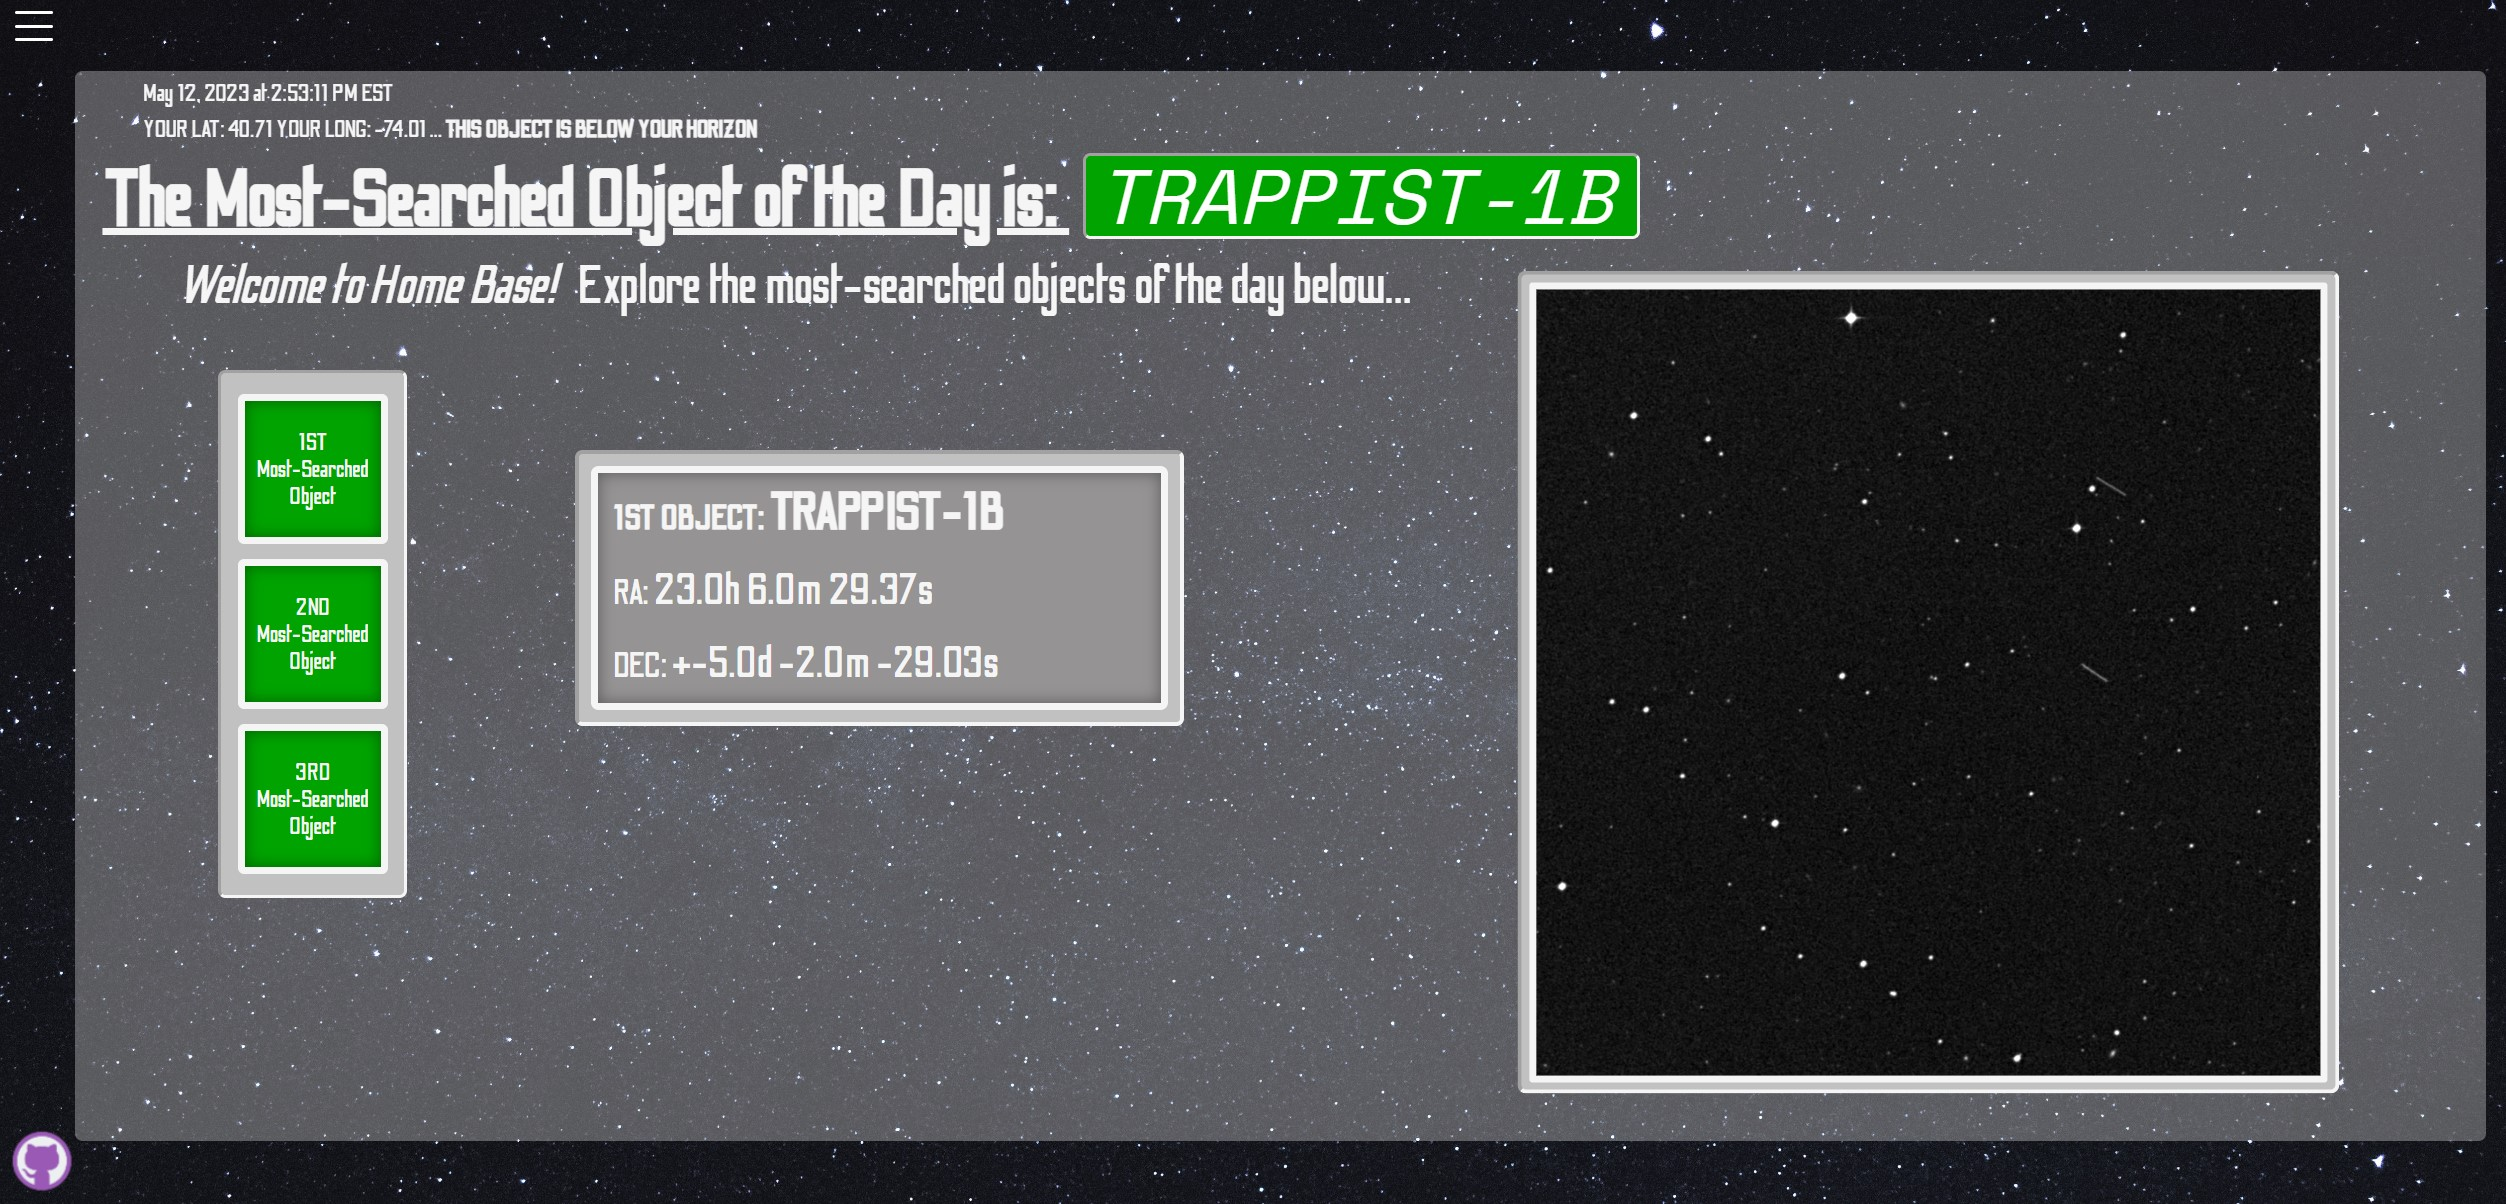
\includegraphics[width=0.9\textwidth]{page1.jpg}
\end{figure}
\begin{figure}[h]
\caption{The interface when user clicks the second button on the left-hand side, prompting 2nd most popular object}
\centering
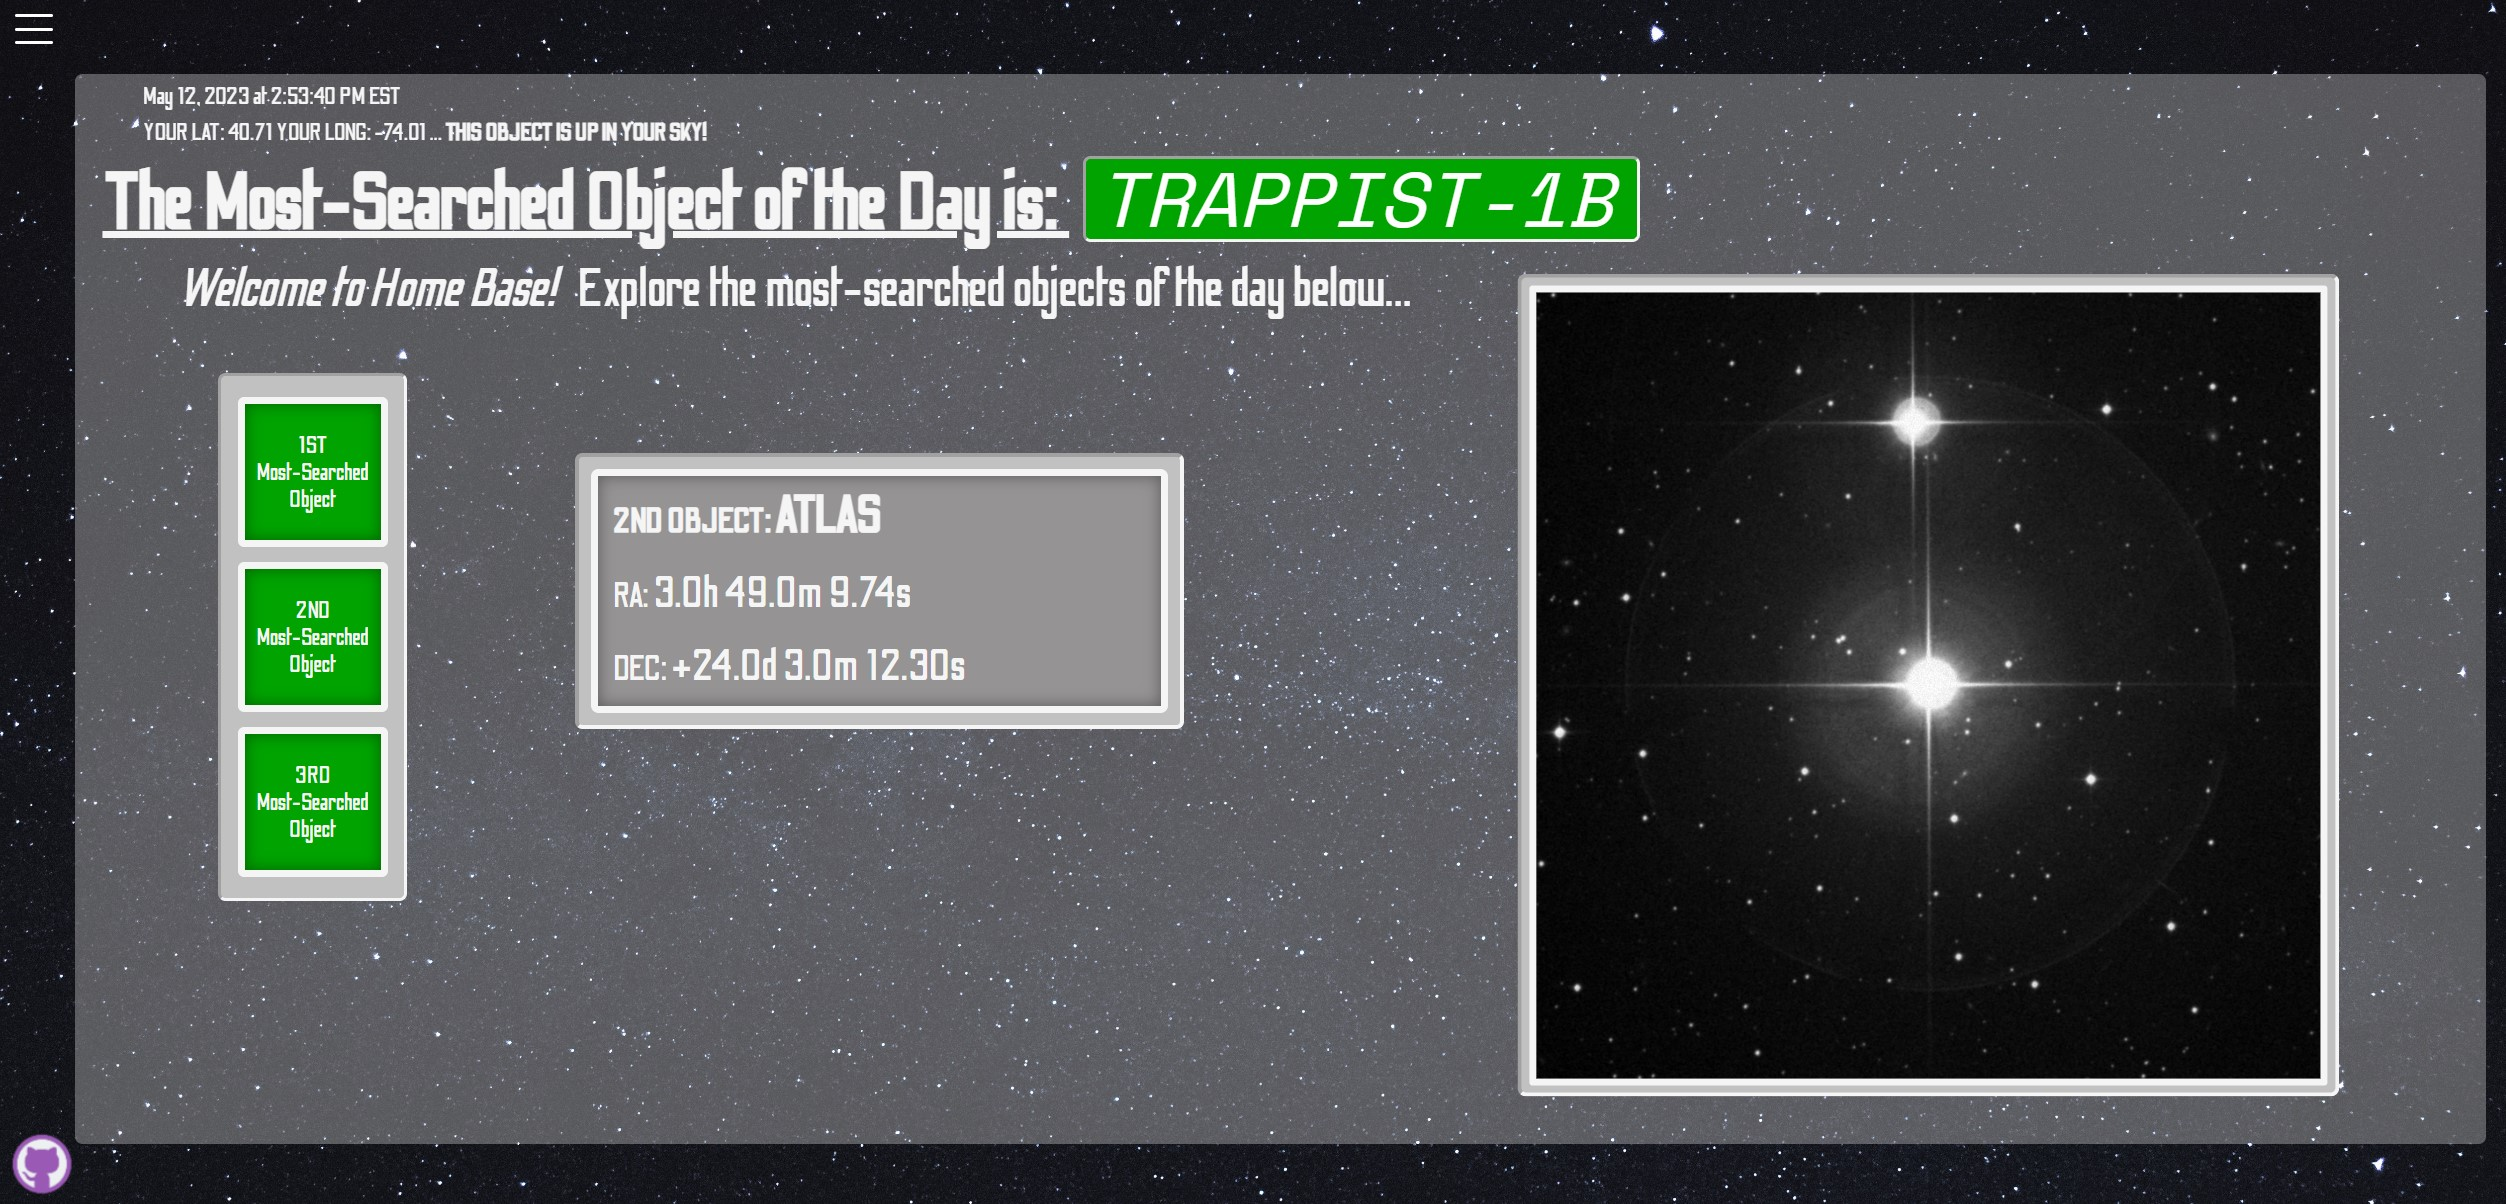
\includegraphics[width=0.9\textwidth]{page2.jpg}
\end{figure}
\begin{figure}[h]
\caption{The interface when user clicks the third button on the left-hand side, prompting 3rd most popular object}
\centering
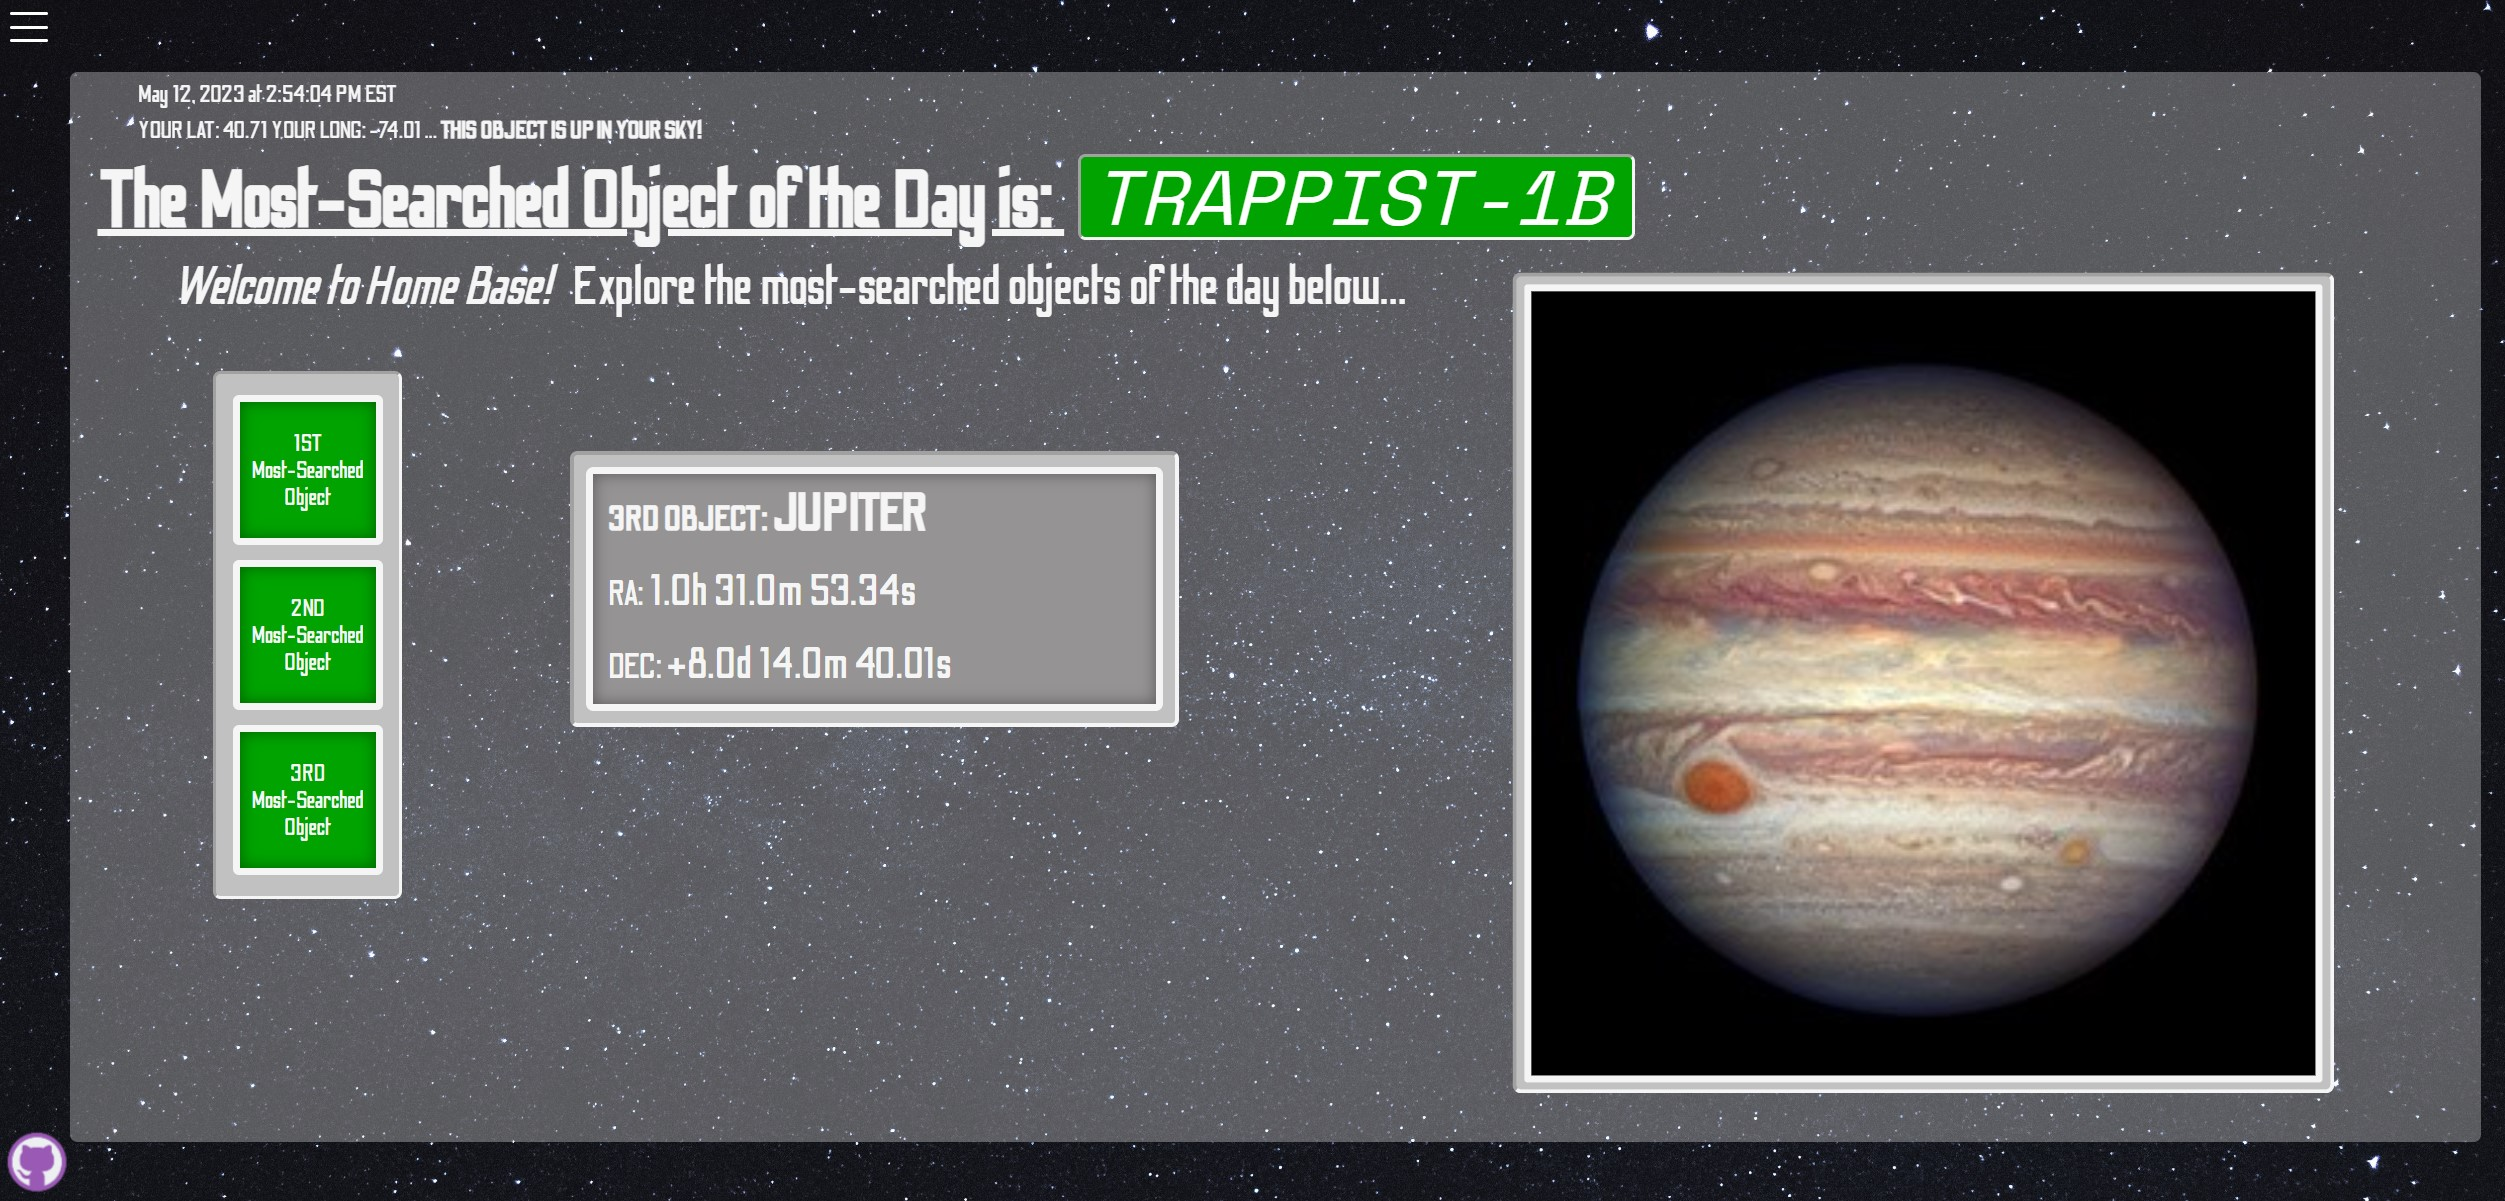
\includegraphics[width=0.9\textwidth]{page3.jpg}
\end{figure}
\\

\\

\subsection*{Project Goals:}
\quad The goal of this project is to automate the process of retrieving popular stellar objects 
from space news websites, analyzing them, and quickly determining the most popular ones to 
observe. We argue that because the popular objects in question are popular amongst
verifiable space news sources, they themselves are promising sources astronomically. 
The project aims to achieve this goal by utilizing advanced techniques in AI and 
automation.\\

\quad The first objective of the project is to develop a web scraping tool that can 
crawl popular space news websites and retrieve articles related to stellar objects. 
The tool will then use natural language processing techniques to identify and extract 
the names of the stellar objects mentioned in the articles.\\

\quad The second objective is to analyze the data collected by the web scraping tool 
to determine the most popular stellar objects among the articles retrieved. This 
will be achieved by using natural language processing to tag keywords mentioned 
in headlines to process the data and identify most mentioned objects in the articles.\\

\quad The third objective is to search for the popular stellar objects identified in 
the second objective within the Space Telescope Science Institute (STScI) database 
using regular expression names. The tool will retrieve the  International 
Celestial Reference System (ICRS) coordinates of the objects, their images, 
and related articles/research papers from the STScI database.\\

\quad The final objective is to present the data retrieved in a user-friendly interface 
that allows astronomers to quickly identify the most popular and promising stellar 
objects to observe. The interface will provide users with a dashboard that displays 
the ICRS coordinates, images, and related articles/research papers of the popular 
stellar objects.\\

\quad Overall, the project aims to streamline the process of identifying and observing 
popular stellar objects by automating the data retrieval and analysis process. 
By achieving these objectives, the project will enable astronomers to make more 
efficient use of their time and resources and increase the likelihood of making 
groundbreaking discoveries in the field of astronomy.\\

\medskip
\printbibliography

\end{document}

